\section{Local Field Potentials}
\ghnote{Torbjorn will write this chapter}

\subsection{Single-neuron LFPs}
\begin{itemize}
\item Passive dendrites \citep{Linden2010}
\item Active dendrites \citep{Ness2016}
\end{itemize}

\begin{figure}[!ht]
\begin{center}
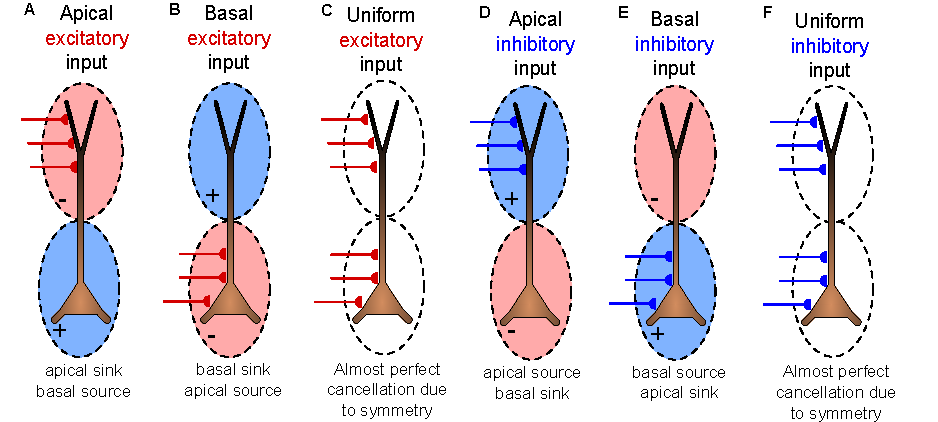
\includegraphics[width=1.\textwidth]{Figures/dipole_basics.pdf}
\end{center}
\caption{\textbf{Basic building blocks of the LFP.}
Illustration of the LFP at a snapshot in time in a region around a pyramidal
cell in response to different types of synaptic input. The LFP signature depends on the type of synaptic input (excitatory
or inhibitory), and the location (apical, basal, uniform), but also, to a lesser degree, to many other parameters of the cells
and synapses.
}
\label{fig:LFP_lego}
\end{figure}

\subsection{Population LFPs}
\begin{itemize}
\item Passive dendrites 
\begin{itemize}
\item Full simulations \citep{Linden2011,Leski2013}
\item Analytical results~\citep{Einevoll2013a}
\item "Magic" simple formula \citep{Mazzoni2015}
\end{itemize}
\item Active dendrites \citep{Ness2018}
\item Effect of correlations
\item Kernel trick? 
\end{itemize}

\subsubsection{Effect of synaptic correlations}
\begin{figure}[!ht]
\begin{center}
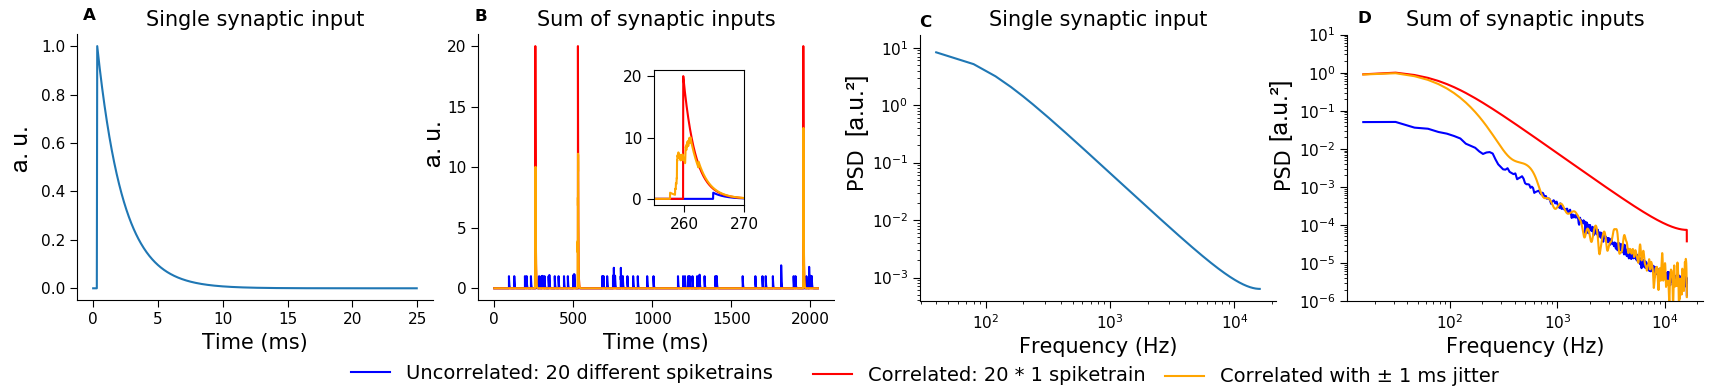
\includegraphics[width=1.\textwidth]{Figures/LFP_effect_correlation_illustration.png}
\end{center}
\caption{\textbf{Illustration of why correlation in synaptic input boosts LFP.}
Basically, it is just because PSD is squared, and variability increase sum of squares: $(1+3) = (2 +2)$, but $(1^2 + 3^2) > (2^2 + 2^2)$
}
\label{fig:correlation_boost}
\end{figure}


\subsection{Network LFPs}
\begin{itemize}
\item Cortical LFPs from single corticothalamic neuron \citep{Hagen2017}
\item Cortical networks with passive dendrites with hybrid trick \citep{Hagen2016}
\item Cortical network with active dendrites \citep{Reimann2013}
\end{itemize}

\subsection{Insights from LFP studies} 
